\subsection{Tranformations}
\dfont{Transformations} are operations we can apply to a function in order to obtain a \ifont{new} function.
The most common transformations include translations, stretches and reflections.
We summarize these below.

\begin{center}
\framebox{
$\begin{array}{ccccl}
\mbox{\underline{Function}}&\qquad&\mbox{\underline{Conditions}}&\qquad&\mbox{\underline{How to graph $F(x)$ given the graph of $f(x)$}}\\
F(x)=f(x)+c&\qquad&c>0&\qquad&\mbox{Shift $f(x)$ upwards by $c$ units}\\
F(x)=f(x)-c&\qquad&c>0&\qquad&\mbox{Shift $f(x)$ downwards by $c$ units}\\
F(x)=f(x+c)&\qquad&c>0&\qquad&\mbox{Shift $f(x)$ to the left by $c$ units}\\
F(x)=f(x-c)&\qquad&c>0&\qquad&\mbox{Shift $f(x)$ to the right by $c$ units}\\
\hline
F(x)=-f(x)&\qquad&~&\qquad&\mbox{Reflect $f(x)$ about the $x$-axis}\\
F(x)=f(-x)&\qquad&~&\qquad&\mbox{Reflect $f(x)$ about the $y$-axis}\\
\hline
F(x)=|f(x)|&\qquad&~&\qquad&\mbox{Take the part of the graph of $f(x)$ that lies}\\
~&\qquad&~&\qquad&\mbox{below the $x$-axis and reflect it about the $x$-axis}\\
\end{array}$}
\end{center}

For horizontal and vertical stretches, different resources use different terminology and notation. 
Use the one you are most comfortable with!
Below, both $a,b$ are positive numbers. Note that we only use the term \ifont{stretch} in this case:

\begin{center}
\framebox{
$\begin{array}{ccccl}
\mbox{\underline{Function}}&\qquad&\mbox{\underline{Conditions}}&\qquad&\mbox{\underline{How to graph $F(x)$ given the graph of $f(x)$}}\\
F(x)=af(x)&\qquad&a>0&\qquad&\mbox{Stretch $f(x)$ vertically by a factor of $a$}\\
F(x)=f(bx)&\qquad&b>0&\qquad&\mbox{Stretch $f(x)$ horizontally by a factor of $1/b$}\\
\end{array}$}
\end{center}

In the next case, we use both the terms \ifont{stretch} and \ifont{shrink}.
We also split up vertical stretches into two cases ($0<a<1$ and $a>1$), and split up horizontal stretches into two cases ($0<b<1$ and $b>1$).
Note that having $0<a<1$ is the same as having $1/c$ with $c>1$.
Also note that \ifont{stretching by a factor of $1/c$} is the same as \ifont{shrinking by a factor $c$}.

\begin{center}
\framebox{ 
$\begin{array}{ccccl}
\mbox{\underline{Function}}&\qquad&\mbox{\underline{Conditions}}&\qquad&\mbox{\underline{How to graph $F(x)$ given the graph of $f(x)$}}\\
F(x)=cf(x)&\qquad&c>1&\qquad&\mbox{Stretch $f(x)$ vertically by a factor of $c$}\\
F(x)=(1/c)f(x)&\qquad&c>1&\qquad&\mbox{Shrink $f(x)$ vertically by a factor of $c$}\\
F(x)=f(cx)&\qquad&c>1&\qquad&\mbox{Shrink $f(x)$ horizontally by a factor of $c$}\\
F(x)=f(x/c)&\qquad&c>1&\qquad&\mbox{Stretch $f(x)$ horizontally by a factor of $c$}\\
\end{array}$}
\end{center}

Some resources keep the condition $0<c<1$ rather than using $1/c$.
This is illustrated in the next table.

\begin{center}
\framebox{
$\begin{array}{ccccl}
\mbox{\underline{Function}}&\qquad&\mbox{\underline{Conditions}}&\qquad&\mbox{\underline{How to graph $F(x)$ given the graph of $f(x)$}}\\
F(x)=df(x)&\qquad&d>1&\qquad&\mbox{Stretch $f(x)$ vertically by a factor of $d$}\\
F(x)=df(x)&\qquad&0<d<1&\qquad&\mbox{Shrink $f(x)$ vertically by a factor of $1/d$}\\
F(x)=f(dx)&\qquad&d>1&\qquad&\mbox{Shrink $f(x)$ horizontally by a factor of $d$}\\
F(x)=f(dx)&\qquad&0<d<1&\qquad&\mbox{Stretch $f(x)$ horizontally by a factor of $1/d$}\\
\end{array}$}
\end{center}

\begin{example}{Transformations and Graph Sketching}{TransformationsGraphSketching}
In this example we will use appropriate transformations to sketch the graph of the function $y=|\sqrt{x+2}-1|-1$.
\end{example}
\begin{solution} 
We start with the graph of a function we know how to sketch, in particular, $y=\sqrt{x}$:
To obtain the graph of the function $y=\sqrt{x+2}$ from the graph $y=\sqrt{x}$, we must shift $y=\sqrt{x}$ to the left by $2$ units.
To obtain the graph of the function $y=\sqrt{x+2}-1$ from the graph $y=\sqrt{x+2}$, we must shift $y=\sqrt{x+2}$ downwards by $1$ unit.
$$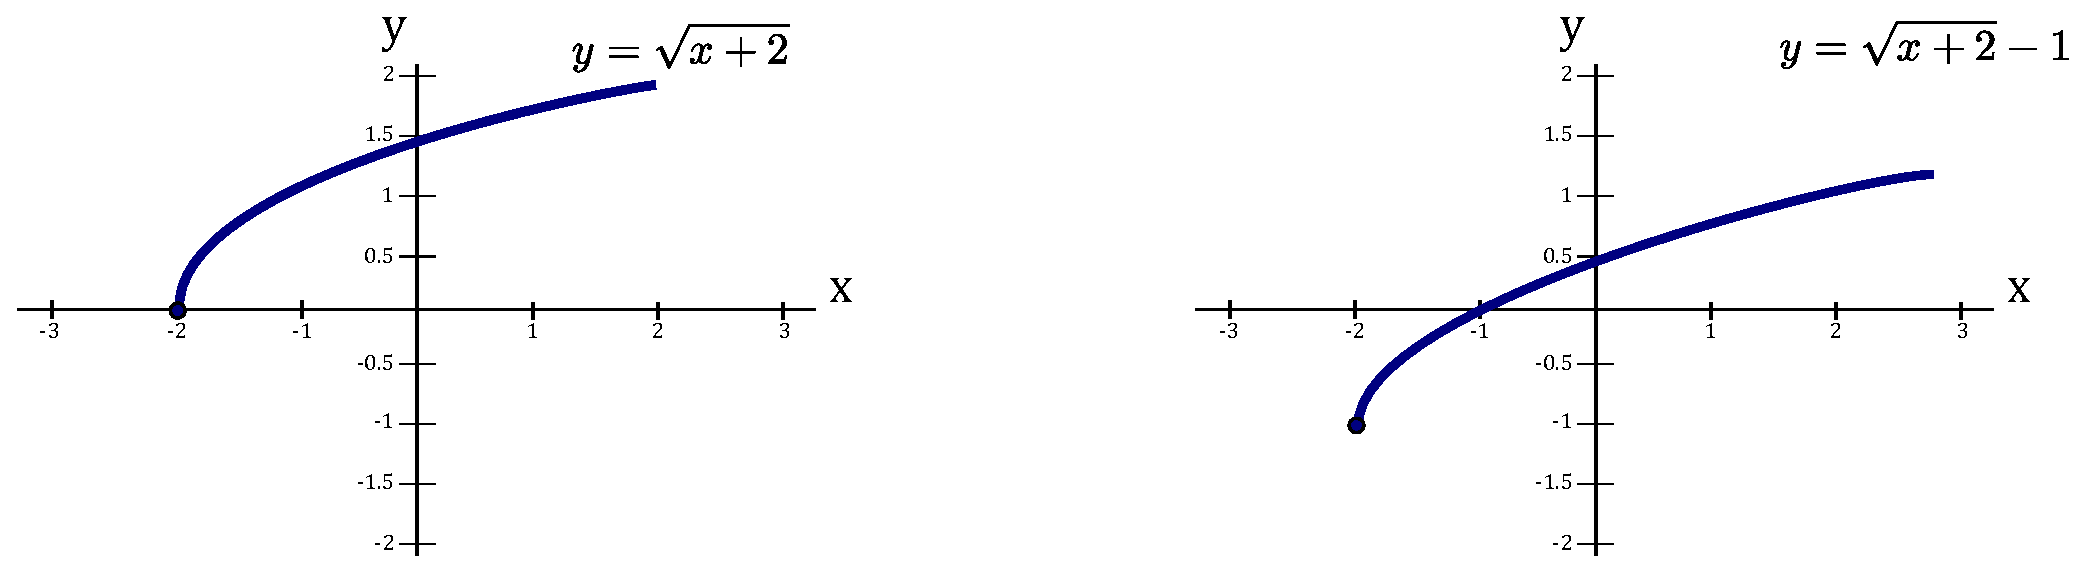
\includegraphics[width=6in]{images/transf1}$$
To obtain the graph of the function $y=|\sqrt{x+2}-1|$ from the graph $y=\sqrt{x+2}-1$, we must take the part of the graph of $y=\sqrt{x+2}-1$ that lies below the $x$-axis and reflect it (upwards) about the $x$-axis.
Finally, to obtain the graph of the function $y=|\sqrt{x+2}-1|-1$ from the graph $y=|\sqrt{x+2}-1|$, we must shift $y=|\sqrt{x+2}-1|$ downwards by $1$ unit:
$$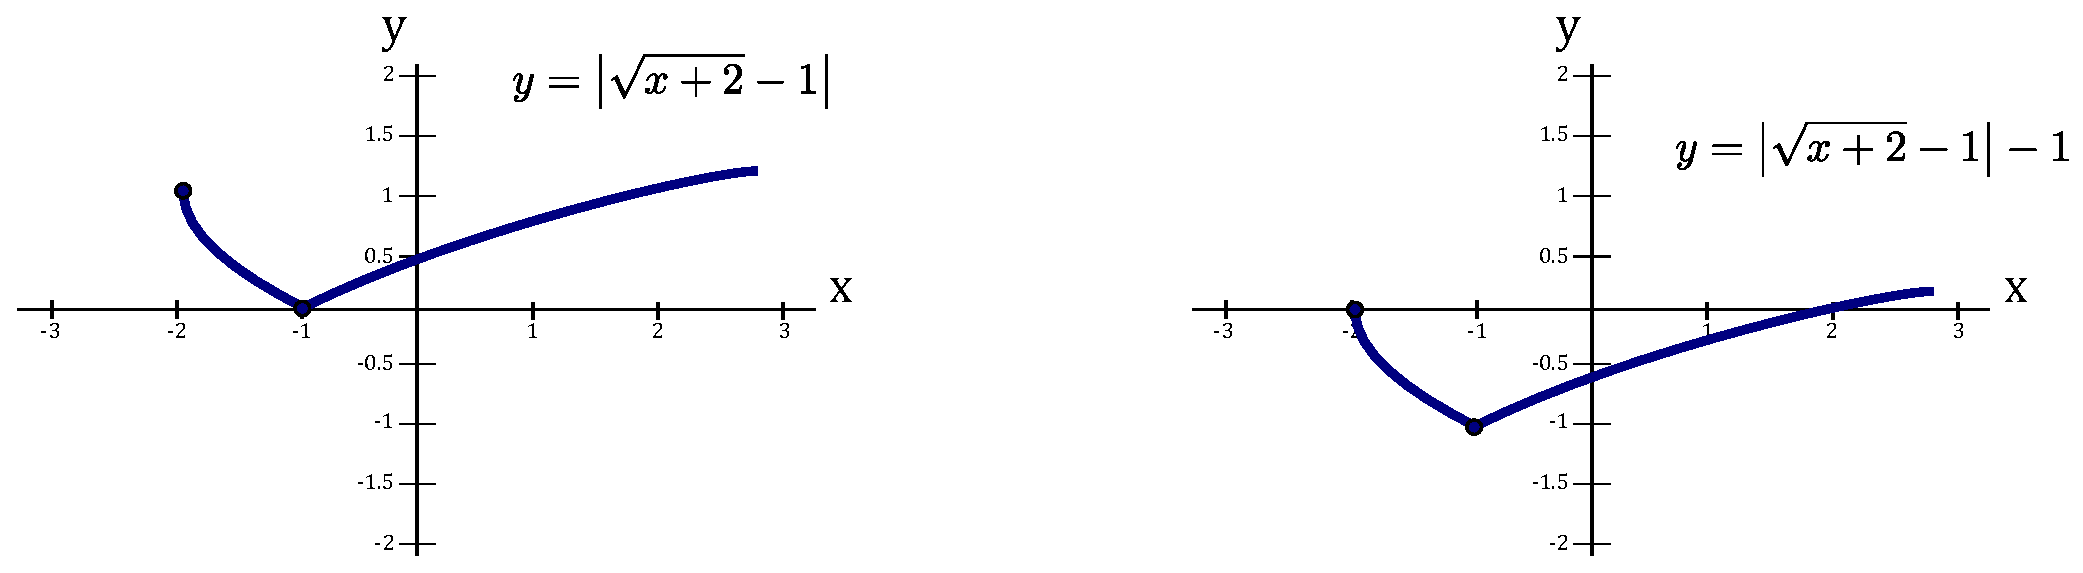
\includegraphics[width=6in]{images/transf2}$$
\end{solution}